\section{Zadání}

\begin{enumerate}
    \item Rešerše statistického párování + PSM.
    \item Pochopení PSM, tzn. jak matematicky funguje, jaké má předpoklady/limitace. V jakých situacích se (ne)hodí.
    \item Vyzkoušení na ostrých datech.
\end{enumerate}

\section{Vypracování}

\subsection{Statistické párování}

Párování (v angl. \enquote*{matching}) je statistická technika používaná k vyhodnocování efektu léčby porovnáním léčených a neléčených pacientů.
Byla vyvinuta s cílem provádět observační studie stejně jako randomizované studie.
Cílem párovacích metod je nalézt pro každého léčeného pacienta jednoho nebo více neléčených pacientů s podobným stavem oproti kterým lze evaluovat efekty léčby.
Premisou takového postupu je umožnit odhadnout reálné účinky léčby a současně redukovat vzniklý statistický bias.

Jak již bylo zmíněno, hlavní myšlenkou je spojit jednotlivé pozorované subjekty ve skupině podstupující léčbu \( A = 1 \) s podobnými jedinci v kontrolní skupině \( A = 0 \) (obecně nepodstupující léčbu, či~podstupující léčbu jinou).
Podobnost jedinců je určena skrze matici příznaků (čili kovariátů) \( X \).
Takovým přístupem získáme zdání kauzality dostatečné v takové míře, že je lze za kauzalitu považovat.

Jakmile jsou data spárována, lze s nimi zacházet jako s randomizovanou studií.
Nevýhodou přístupu je, že obvykle nelze pracovat s celou maticí příznaků.
Práce s kompletní maticí příznaků je vhodná pro úlohu klasifikace, kdy se snažíme jednoznačně odlišit jednu skupinu od druhé.
To ale není pro párování příliš praktické.
V této úloze naopak hledáme matici příznaků takovou, které nám umožní najít znatelný překryv.
Právě v překryvu dvou skupin lze hledat entity vhodné pro párování.

\begin{figure}[htbp]
	\centering
	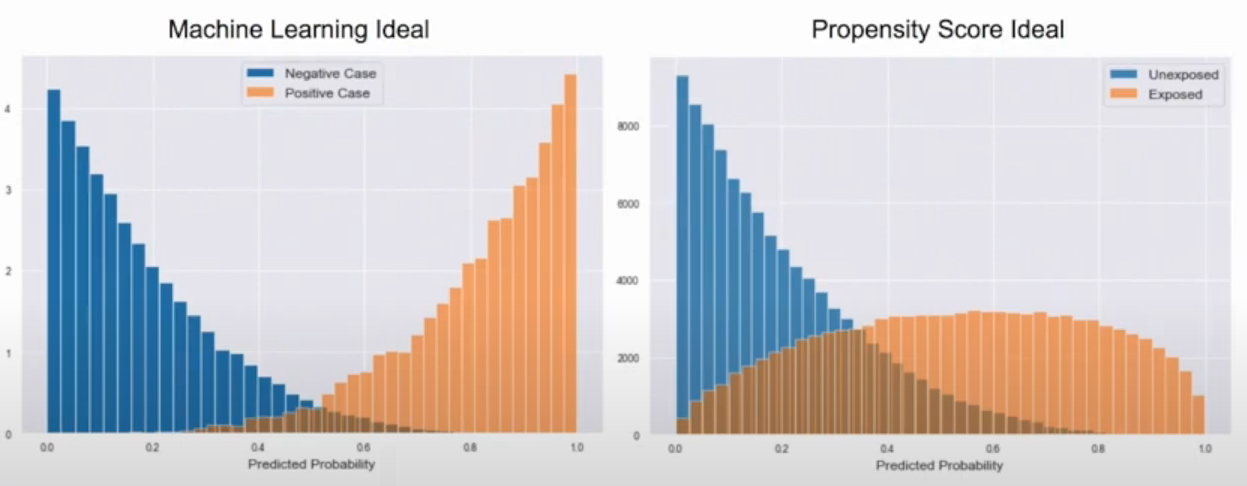
\includegraphics[width=0.9\textwidth]{graphs/psm-vs-class.png}
	\caption{Klasifikace vs PSM}
\end{figure}
\FloatBarrier

Při provádění metod statistického párování postupujeme tedy následovně:

\begin{enumerate}
    \item data rozdělíme na dvě skupiny, kontrolní a experimentální; kontrolní je obvykle větší;
    \item vybereme příznaky, které budou použity pro výpočet skóre podobnosti;
    \item vypočteme skóre podobnosti (logistickou regresí, či jinou metodou);
    \item dle skóre z předešlého kroku spárujeme prvky z kontrolní a experimentální skupiny (například pomocí algoritmu pro hledání nejbližšího souseda).
\end{enumerate}

Výběr příznaků pro metodu PSM je volbou analytika v závislosti na konkrétní situaci.
Jak již bylo zmíněno výše, je nutné zvolit takové příznaky, které umožní najít jistý překryv kontrolní a léčené skupiny.

Při výpočtu skóre náchylnosti je výchozí volbou \textit{logistická regrese}.
Použití jiných metod záleží (stejně jako u \textit{výběru příznaků}) pouze na analytikovi a dané situaci.
V článku \enquote{Propensity score estimation: machine learning and classification methods as alternatives to logistic regression} z roku 2010 popisují autoři použití i neuronových sítí, SVM a rozhodovacích stromů.
Nejčastější alternativní volbou by byl pravděpodobně Bayesův klasifikátor.
Ten podle článku \enquote{Bayesian propensity score analysis for observational data} z roku 2009 bude lepší volbou obzvláště v případech, kdy se v datech nachází nějaká míra nejistoty.

Při párování se pro každý prvek experimentu hledá prvek v kontrolní skupině.
Implicitně se předpokládá, že kontrolní skupina je početnější, jelikož léčba je obvykle nákladná nebo nemoc vzácná.
Otázka nastává, co dělat s případy, kdy je kontrolní skupina menší než léčená (což nastává i v naší situaci).
V takových případech je metoda PSM stále validní možností, protože úloha není nutně o~hledání párů dat, ale spíše o~hledání dvou srovnatelných skupin dat.
Toho i v tomto \enquote{inverzním} případě dosáhneme (ani se nemění směr párování).
Dle dostupných informací na fórech je však rozumné uvážit (a nastudovat) i další metody, jako např. \textit{Coarsened Exact Matching}, které v takových případech mohou být někdy vhodnější.

\subsubsection{Kovariát (covariate)}

Kovariáty jsou charakteristikami účastníků experimentu (jejich vlastnosti, vyjma vlastní léčby), tedy jedná se o matici příznaků \( X \).
Mějme experiment zkoumající vliv antihypertenziv (léků snižujících krevní tlak) při léčbě posttraumatické stresové poruchy (PTSP) vyskytující se u válečných veteránů.
Míra dávky léku je v tomto kontextu léčbou, zatímco věk a další biologické rysy (váha, výška) jsou faktory ovlivňující výkonnost léčby, jsou tedy kovariáty léčby.

\subsection{Ohodnocení podobnosti subjektů}

Abychom mohli realizovat cíl \textit{statistického párování} potřebujeme nejdříve nadefinovat nějakou metriku, dle které půjde zhodnotit podobnost jednoho subjektu k subjektu druhému.
Asi nejjednodužší metrikou jsou \textit{propensity scores}, v překladu skóre náchylnosti či sklonu.

Již jsme definovali experimentální množinu subjektů \( A = 1 \) a kontrolní skupinu \( A = 0 \).
\enquote{Propensity score} \( \pi \) pro subjekt \( i \) definujme jako pravděpodobnost příslušnosti subjektu do experimentální skupiny.

\[ \pi_i = P(A = 1 | X_i) \]

Uveďme příklad, jestliže je skóre subjektu \( 0.3 \), pak to znamená, že na základě matice vektoru příznaků má \( 30\% \) šanci, že spadá do experimentální skupiny (často označováno jako skupina \textit{léčba}).
Toto skóre je možné získat jakýmkoliv klasifikačním algoritmem (samozřejmě upraveným tak, aby nevracel jen třídu, ke skteré si myslí, že prvek náleží, ale i regresní složku, tedy procentuální příslušnost).
Tady lze využít např. \textit{logistickou regresi}.

\subsubsection{Redukce biasu}

Přes pečlivý výběr konkrétních příznaků, které budou pro párování použity, se pravděpodobně nepovede vybrat příznaky zcela vyvážené (nezatížené biasem).
Nevyváženost příznaků bohužel v této metodě způsobuje, že nedojde k dostatečnému podobnostnímu překryvu párovaných skupin.
Potřebujeme tedy výpočet, díky kterému zjistíme které příznaky způsobují imbalanci.
To lze zjistit pomocí \enquote*{standardized mean difference} (\textit{smd}), tedy pomocí \textit{standardizovaných odchylek od průměru}.
Výpočet \textit{smd} je rozdílem středních hodnot mezi dvěma skupinami, vyděleným sdruženou směrodatnou odchylkou.

\[ smd = \frac{\bar{X}_t - \bar{X}_c}{ \sqrt{\frac{(s^2_t + s^2_c)}{2} }} \]

Spočítáme \textit{smd} pro každý příznak.
Pro určení, jestli je příznak vyvážený, nebo ne, se použije následující pravidlo:

\begin{itemize}
	\item \( smd < 0.1 \) ideální stav,
	\item \( smd \in (0.1-0.2) \), hraniční stav,
	\item \( smd > 0.2 \), vážně nevyvážený případ.
\end{itemize}

V ideálním případě jsou hodnoty \textit{smd} rovny prvnímu případu, tedy do \( 0.1 \).
Mnohdy tomu ale tak není, tento problém má několik řešení.

\paragraph{První řešení}

je odstranit entity s extrémními hodnotami \textit{propensity score}.
Odstraníme tedy subjekty, jejichž skóre je menší než minimum z \textit{léčené} skupiny a jejichž skóre je větší než maximum z kontrolní skupiny a \textit{vice versa}.

\paragraph{Druhé řešení}

je vzít v úvahu pouze takové dvojice subjektů (z kontrolní a experimentální skupiny), u~nichž je rozdíl podobnostní metriky menší než specifikovaná mez \( \delta \).

\paragraph{Třetí řešení}

je použito v kódu dodaného spolu s tímto textem.
Jedná se o řešení, kdy subjekt z~experimentální skupiny je spárován s několika sousedy z druhé skupiny (kNN).

\subsection{Ověření hypotéz}

V rámci implementace PSM byli na datech ověřeny 2 hypotézy.
První hypotézou \( H_1 \) je, že provedení léčebných postupů vede ke snížení NIHSS sledovaných pacientů.
Hypotézy byly definovány následovně:

\begin{itemize}
    \item $H_0$: provedení léčebných postupů (Trombectomie, Trombolýza, Bridge) \textit{nevede} ke snížení NIHSS sledovaných pacientů;
    \item $H_A$: provedení léčebných postupů \textit{vede} ke snížení NIHSS sledovaných pacientů.
\end{itemize}

Druhou ověřovanou hypotézou \( H_2 \) bylo, že u pacientů ve věku do 65 let provedení léčebných postupů vede ke snížení NIHSS většímu než u pacientů nad 65 let.

\begin{itemize}
    \item $H_0$: u pacientů ve věku do 65 let provedení léčebných postupů (Trombectomie, Trombolýza, Bridge) \textit{nevede} ke snížení NIHSS ve srovnání s pacienty nad 65 let;
    \item $H_A$: u pacientů ve věku do 65 let provedení léčebných postupů \textit{vede} ke snížení NIHSS sledovaných pacientů ve srovnání s pacienty nad 65 let.
\end{itemize}

V obou případech se podařilo T-testem zamítnout nulovou hypotézu na úrovni hladiny \( \alpha = 5 \: \% \) a~přijmout hypotézu alternativní.

\begin{table}[htbp]
    \centering

    \begin{tabular}{@{}lllcc@{}}
        \toprule
                    & Statistika & p-value         & Velikost kontrolní skupiny    & Velikost exponované skupiny   \\ \midrule
        \( H_1 \)  & -7.99      & \num{2.6e-15}   & 1312                          & 1578                          \\
        \( H_2 \)  & -5.63      & \num{2.3e-8}    & 385                           & 1193                          \\
        \bottomrule
    \end{tabular}

\end{table}
\FloatBarrier

Dle výsledků statistik z tabulky výše můžeme vyvodit, že léčení pacienta (první hypotéza) vede ke znatelnému snížení NIHSS (znaménko mínus ve statistice lze v tomto případě interpretovat jako snížení NIHSS).
U druhé hypotézy můžeme soudit obdobně.

Datasetu obsahuje celkem 2890 záznamů.
V první hypotéze uvažujeme celý dataset rozdělený do dvou skupin, přičemž kontrolní skupina obsahuje 1312 záznamů a exponovaná skupina (léčená) obsahuje celkem 1578 záznamů (66 trombektomií, 1251 trombolýz a 261 bridge), pro kontrolu \( 66 + 1251 + 261 = 1578 \) a~\( 1312 + 1578 = 2890 \).
V druhé hypotéze uvažujeme redukovaný dataset, pouze léčených pacientů (celkem 1578 záznamů), rozdělený podle věku pacientů (nad 65 let včetně v počtu 1193 a pod 65 let v počtu 385~pacientů).

Při párování se v uvažovaných hypotézách, kvůli dominanci exponované skupiny, multiplikují prvky z~kontrolních skupin.
Párování proběhne vždy v celém oboru léčené skupiny, je tedy párováno 1578 dvojic pro \( H_1 \) a 1193 dvojic pro \( H_2 \).

\begin{figure}[htbp]
	\centering
	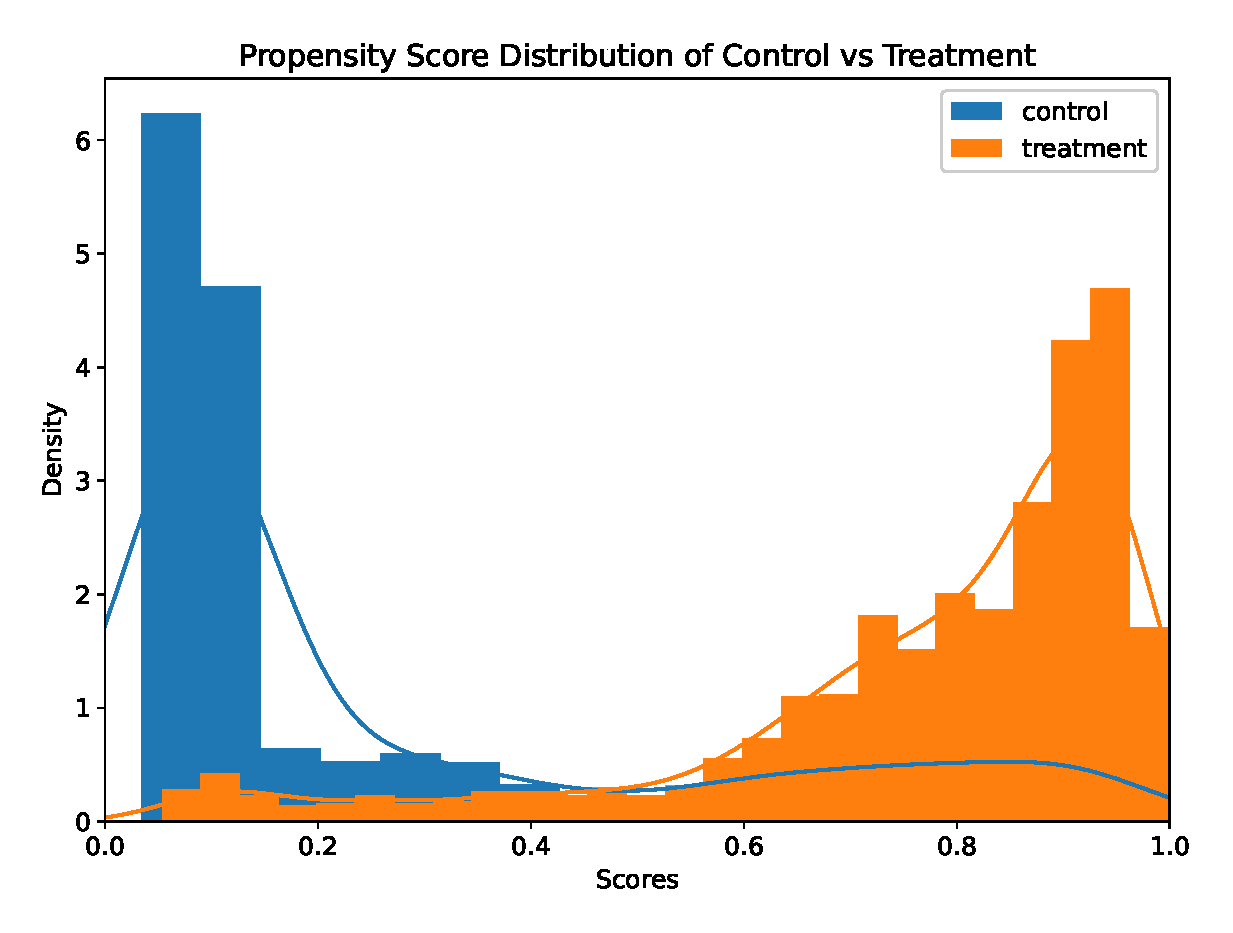
\includegraphics[width=0.6\textwidth]{graphs/h1.eps}
	\caption{Graf Propensity Scores pro \( H_1 \)}
\end{figure}
\FloatBarrier

\begin{figure}[htbp]
	\centering
	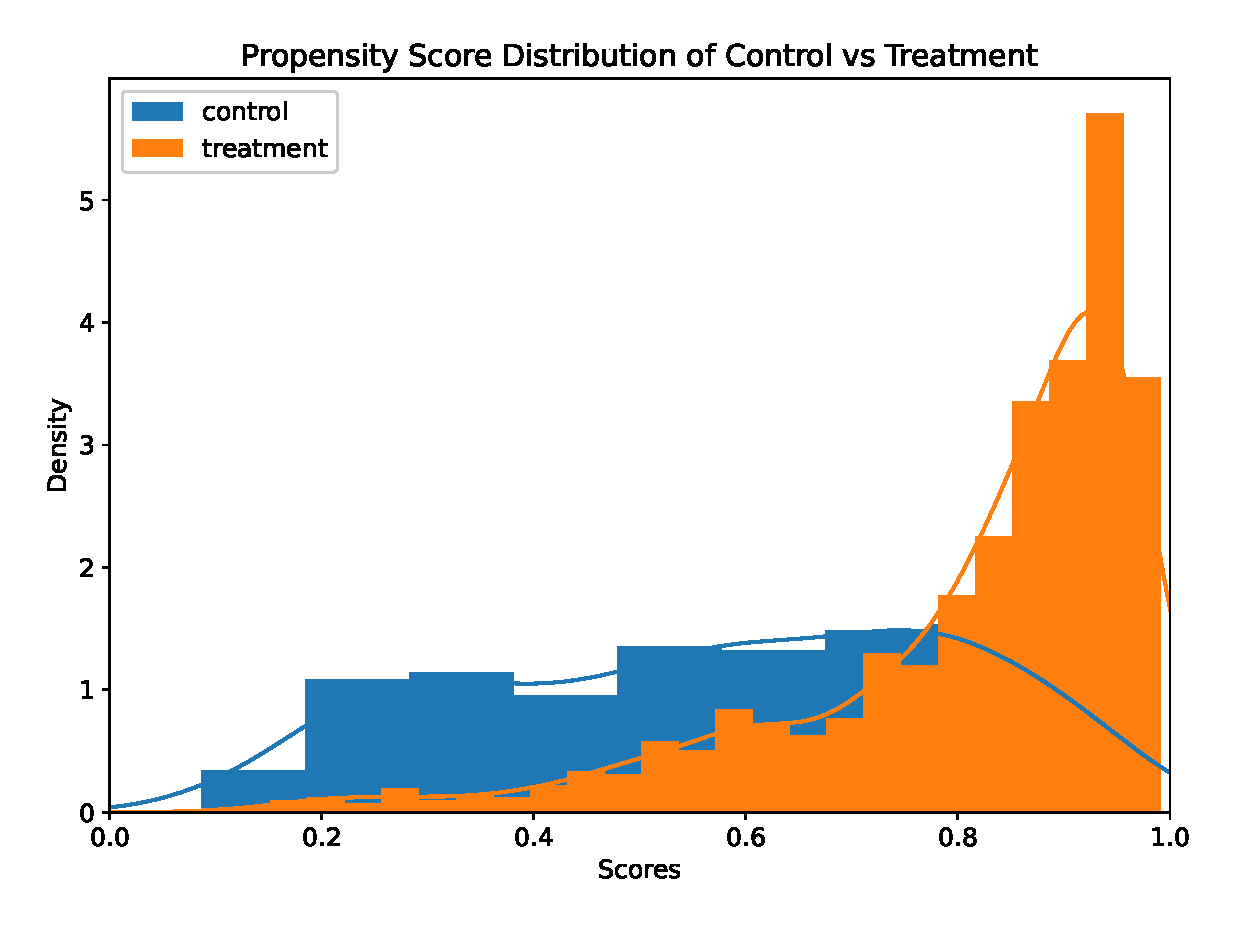
\includegraphics[width=0.6\textwidth]{graphs/h2.eps}
	\caption{Graf Propensity Scores pro \( H_2 \)}
\end{figure}
\FloatBarrier

\section{Závěr}

Ačkoliv je PSM velice efektivní technikou, tak v některých publikacích není doporučována, konkrétně v~článku \enquote{Why Propensity Scores Should Not Be Used for Matching}.
Autoři v tomto článku vysvětlují, kdy je technika PSM používána a proč je tak používána nesprávně.
Prezentují techniky CEM (Coarsened Exact Matching) a MDM (Mahalanobis Discrepancy Matching), které představují alternativu k~PSM dávající v~určitých případech smysluplnější výsledky než PSM.
V těchto případech se však jedná o~\enquote{pouhou} změnu definice podobnosti.

Vcelku se jedná o velice zajímavý statistický nástroj, v principu i snadno pochopitelný.
